\documentclass[russian,utf8,emptystyle]{eskdtext}

\newcommand{\No}{\textnumero} % костыль для фикса ошибки

\ESKDdepartment{Федеральное государственное бюджетное образовательное учреждение высшего профессионального образования}
\ESKDcompany{Московский государственный технический университет им. Н. Э. Баумана}
\ESKDclassCode{23 0102}
\ESKDtitle{Курсовая работа по дисциплине}
\ESKDdocName{<<Эксплуатация АСОИиУ>>}
\ESKDauthor{Гуща~А.~В.}
\ESKDtitleApprovedBy{к.т.н. доцент}{Постников В.М.}
\ESKDtitleAgreedBy{к.т.н. доцент}{Постников В.М.}
\ESKDtitleDesignedBy{Студент группы ИУ5-92}{Гуща~А.~В}

\usepackage{multirow}
\usepackage{tabularx}
\usepackage{tabularx,ragged2e}
\usepackage{pdfpages}
\renewcommand\tabularxcolumn[1]{>{\Centering}p{#1}}
\newcommand\abs[1]{\left|#1\right|}

\usepackage{longtable,tabu}

\usepackage{geometry}
\geometry{footskip = 1cm}

\pagenumbering{arabic}
\pagestyle{plain}

\usepackage{setspace}
\usepackage{enumitem}

\usepackage{xcolor}
\usepackage{listings}
\lstset{
    breaklines=true,
    postbreak=\raisebox{0ex}[0ex][0ex]{\ensuremath{\color{red}\hookrightarrow\space}},
    extendedchars=\true,
    basicstyle=\small,
    inputencoding=utf8
}
\lstdefinelanguage{D}{
    keywords = {
    abstract,
    alias,
    align,
    asm,
    assert,
    auto,
    body,
    bool,
    break,
    byte,
    case,
    cast,
    catch,
    cdouble,
    cent,
    cfloat,
    char,
    class,
    const,
    continue,
    creal,
    dchar,
    debug,
    default,
    delegate,
    delete,
    deprecated,
    do,
    double,
    else,
    enum,
    export,
    extern,
    false,
    final,
    finally,
    float,
    for,
    foreach,
    foreach_reverse,
    function,
    goto,
    idouble,
    if,
    ifloat,
    immutable,
    import,
    in,
    inout,
    int,
    interface,
    invariant,
    ireal,
    is,
    lazy,
    long,
    macro,
    mixin,
    module,
    new,
    nothrow,
    null,
    out,
    override,
    package,
    pragma,
    private,
    protected,
    public,
    pure,
    real,
    ref,
    return,
    scope,
    shared,
    short,
    static,
    struct,
    super,
    switch,
    synchronized,
    template,
    this,
    throw,
    true, 
    try,
    typedef,
    typeid,
    typeof,
    ubyte,
    ucent,
    uint,
    ulong,
    union,
    unittest,
    ushort,
    version,
    void,
    volatile,
    wchar,
    while,
    with,
    __FILE__,
    __MODULE__,
    __LINE__,
    __FUNCTION__,
    __PRETTY_FUNCTION__,
    __gshared,
    __traits,
    __vector,
    __parameters,
    }
}

\begin{document}
\maketitle
%\includepdf[pages={1}]{title.pdf}

\section{Реферат}
\clearpage

\tableofcontents
\clearpage

\section{Техническое задание}
Исходные данные для выполнения курсовой работы представлены в таблице~\ref{tab:task}.

\begin{longtable}{p{1cm}|p{2cm}|p{2cm}|p{2cm}|p{2cm}|p{2cm}|p{1.5cm}|p{1.5cm}}
\caption{Исходные данные для выполнения курсовой работы.}
\label{tab:task} \\
№  & Цент-ральный офис & 1-ый филиал & 2-ой филиал & СУБД и выбор оборудования & Диски сервера & Диски сервера & Модель \\ 
\hline 
8 & 5(1)/2(1) & 3(3)/2(3) & \centering 18 & 23/33/43 & \centering 53 & 64 (5) (0.9) & \centering 73 \\ 
\end{longtable}

\subsection{Наименование}
Проектирование распределённой АСОИиУ фирмы.

\subsection{Основание для разработки}
Основанием для разработки является учебный план кафедры ИУ5 МГТУ им. Н.Э. Баумана.

\subsection{Цель разработки}
Целью разработки является создание проектного решения на распределенную сеть обра-
ботки информации, объединяющую все подразделения фирмы, состоящей из центрального и двух
удаленных офисов.

\subsection{Задачи, подлежащие решению}
В процессе выполнения курсовой работы необходимо решить следующие задачи:
\begin{enumerate}[label=\arabic*.]
\item Разработать блок-схему распределенной АСОИиУ фирмы и структурные схемы ЛВС цен-
трального и удаленных офисов фирмы;
\item Описать правила построения всех сетей фирмы;
\item Выбрать и обосновать вариант удаленной связи отдельных ЛВС фирмы;
\item Выбрать требуемое оборудование для ЛВС фирмы;
\item Описать настройку рабочих параметров сетевой ОС, под управлением которой работают ЛВС
фирмы;
\item Описать настройку рабочих параметров СУБД, которая установлена в ЛВС фирмы;
\item Провести распределение предметных баз данных по узлам сети;
\item Выполнить аналитическое и имитационное моделирование ЛВС фирмы и провести сравни-
тельный анализ результатов моделирования;
\item Разработать и представить рекомендации по модернизации и реорганизации распределенной
АСОИиУ фирмы.
\end{enumerate}


\subsection{Требования к составу технических средств}
Фирма состоит из центрального офиса и двух филиалов.

В центральном офисе фирмы расположены ЛВС 100Base-TX, содержащая один концетратор, и ЛВС 10Base-2, содержащая один сегмент. Обе сети подключены к коммутатору, к нему также подключен удаленный маршрутизатор с двумя модемами. 

В первом филиале фирмы расположены ЛВС 10Base-T, содержащая три концетратора, и ЛВС 10Base-2, содержащая три сегмента. Обе сети подключены к коммутатору, к нему также подключен удаленный маршрутизатор с одним модемом.

Во втором филиале фирмы расположена ЛВС Token Ring на комбинированной среде (ВОЛС (волоконно-оптическая линия связи) и ЭВП (экранированная витая пара)). 

\subsection{Требования к составу программных средств}
ЛВС работает под управлением сетевой ОС Windows Server 2003 и СУБД SQL Server. 

\subsection{Техническая документация, предъявляемая по окончанию работы}
По окончании работы должна быть предъявлена следующая документация:
\begin{enumerate}[label=-]
\item структурная схема объединённой сети фирмы;
\item распределение предметных баз данных по узлам сети;
\item формализованная схема сети и результаты моделирования;
\item пояснительная записка.
\end{enumerate}

\subsection{Порядок приема работы}
Приём работы осуществляется путем проверки соответствия выполненной работы пунктам
технического задания.

\subsection{Дополнительные условия}
В ЛВС установлен сервер на базе двухядерного процессора с дисковой подсистемой RAID-6, содержащая 5 базовых диска (без учета уровня RAID), при условии, что вероятность безотказной работы одного диска равна 0.9 и все диски одинаковые.

Необходимо провести сравнительный анализ серверов отдела на базе двухядерных процессоров  и выбрать наилучший.

Подробно описать особенности эксплуатации  системного блока сервера.

Модель должна позволять проводить ее настройку на два варианта:
\begin{itemize}
\item на общий вид моделируемой ЛВС, чтобы можно было провести исследование любого варианта;
\item на вариант задания (исходные данные - только данные задания). 
\end{itemize}

Результаты моделирования должны соответствовать варианту задания, поэтому  необходимо провести  моделирование системы, содержащей 8 рабочих станций, ПЭВМ, канал и два сервера.

\clearpage
\section{Архитектура объединенной сети фирмы}
\subsection{Общая схема сети}
Объединенная сеть состоит из сети центрального офиса, сети 1 филиала и сети 2 филиала. Её общая схема изображена на рисунке~\ref{fig:network-all}. В графических обозначениях схема изображена на рисунке~\ref{fig:network-all-2}.

\begin{figure}[h!]
\centering
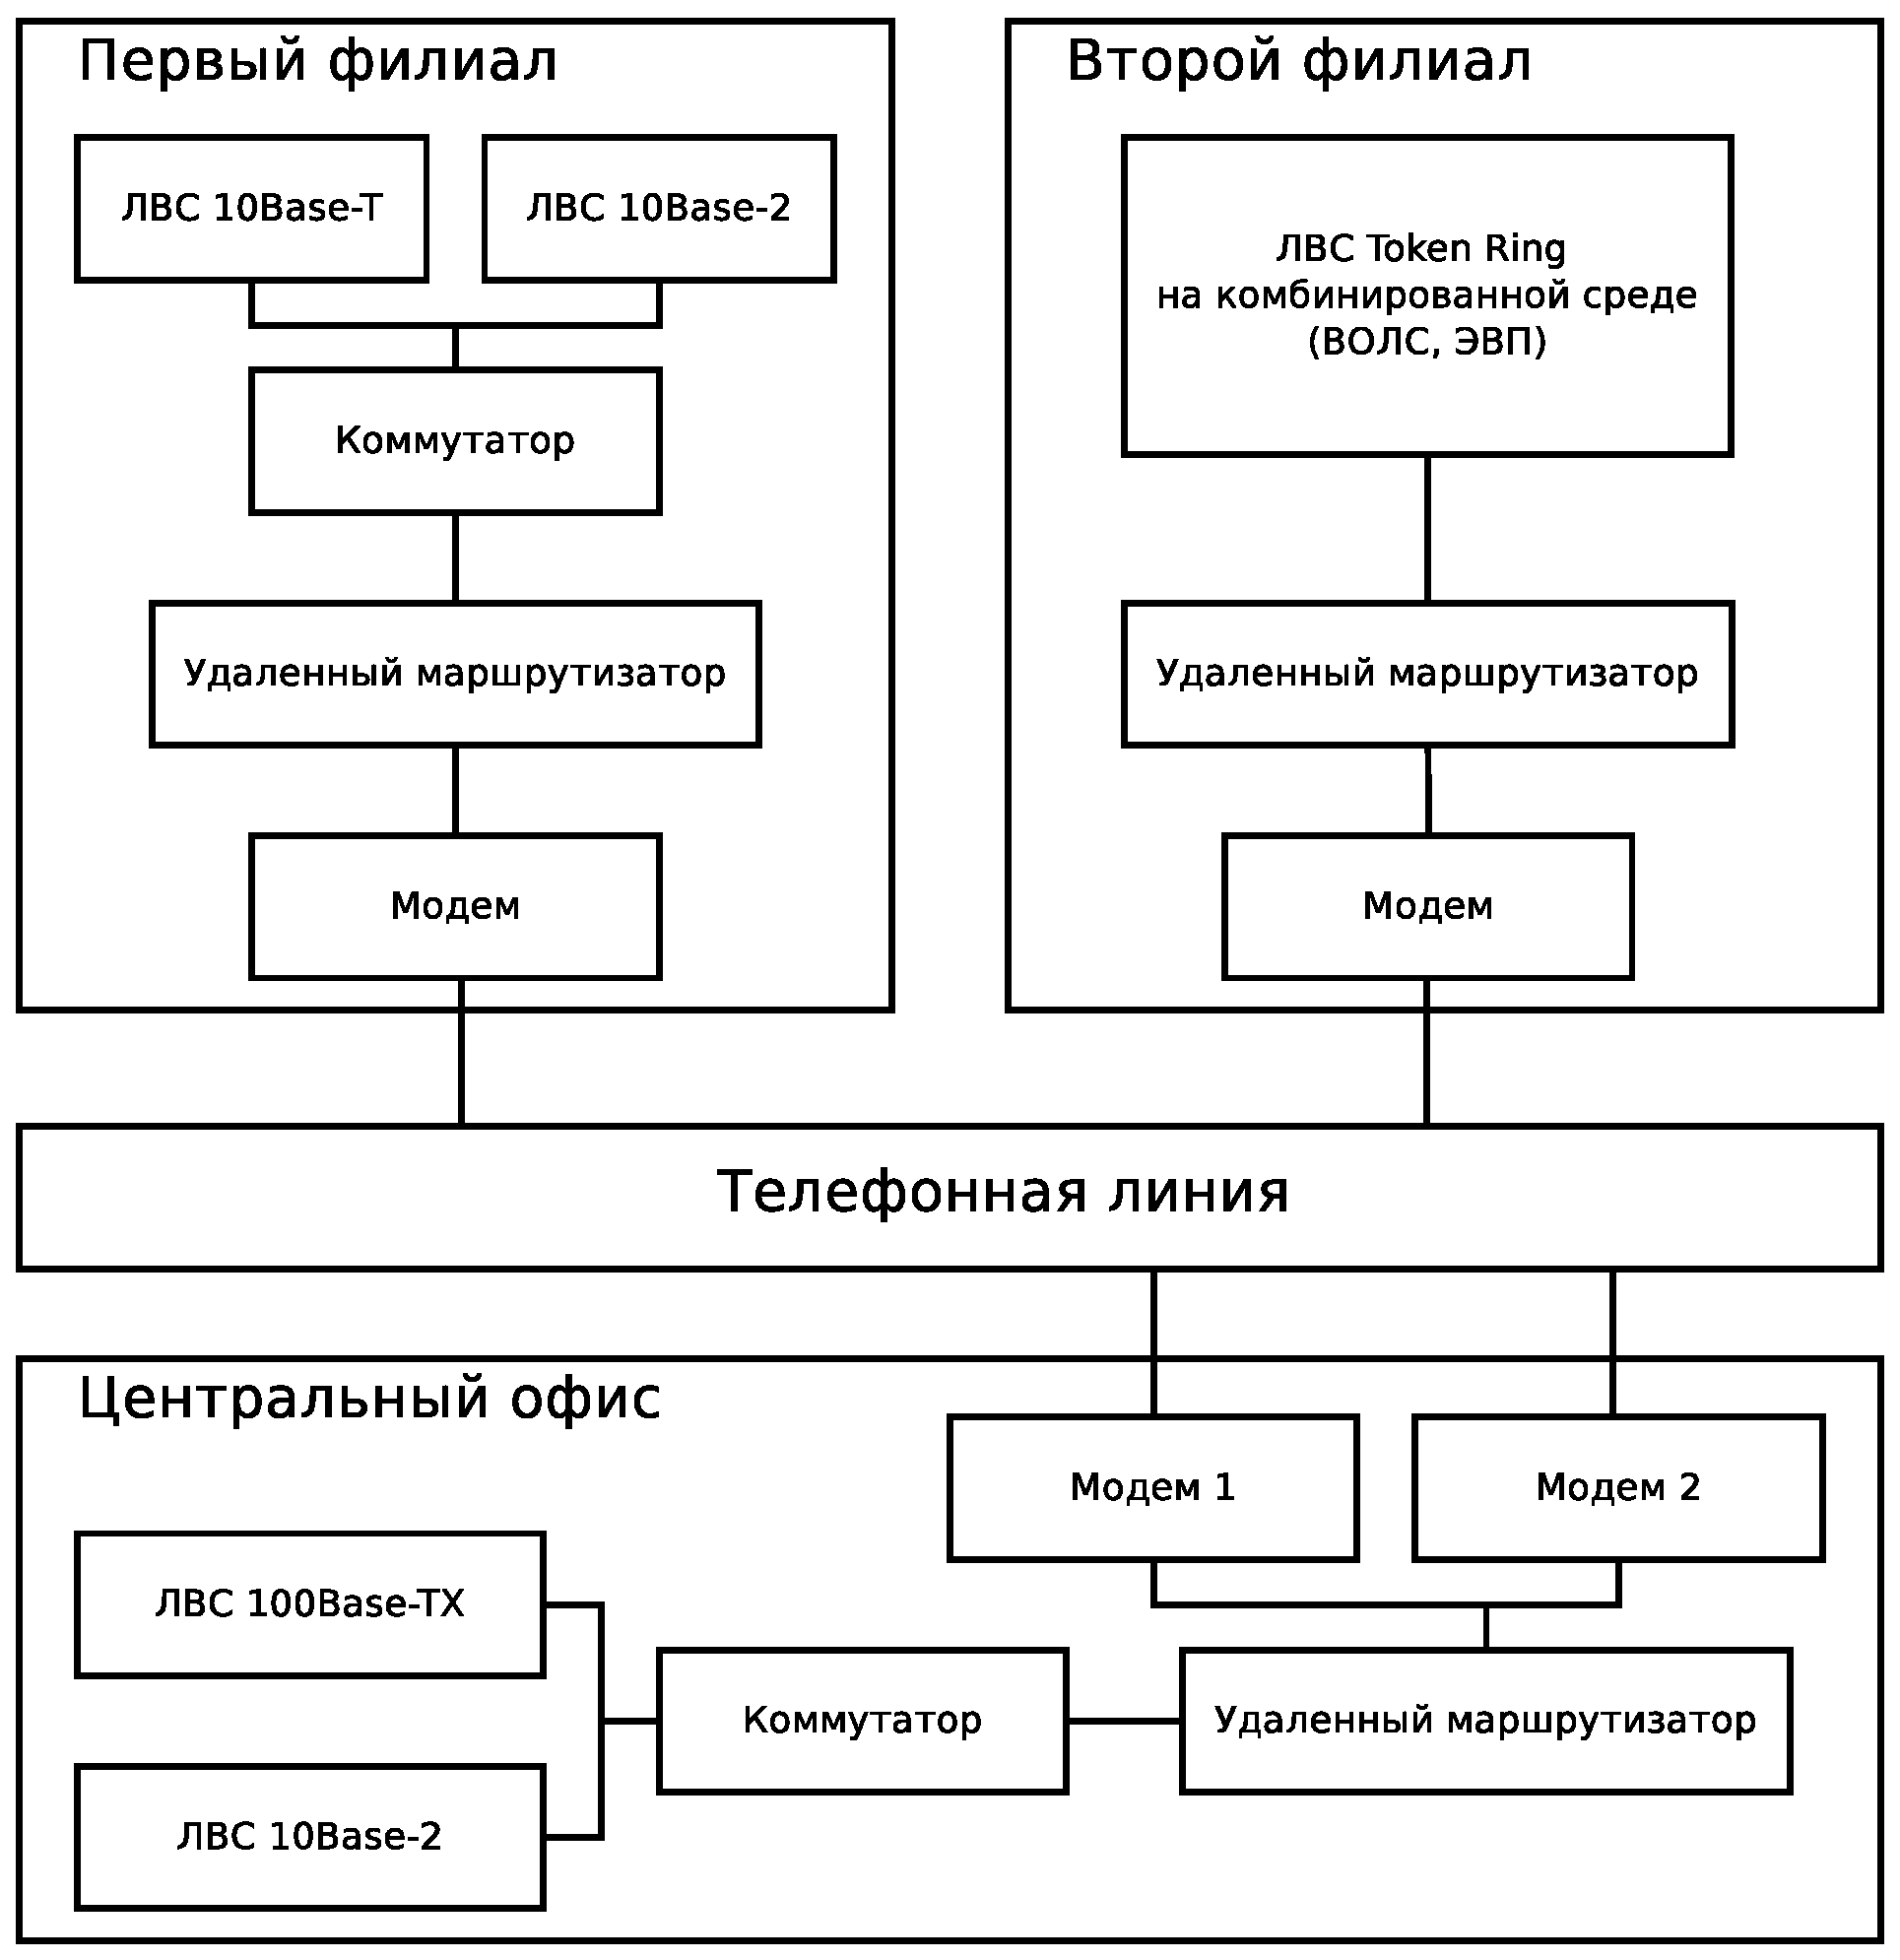
\includegraphics[width = 0.8\textwidth]{network-all}
\caption{Общая схема объединенной сети.}
\label{fig:network-all}
\end{figure}

В центральном офисе фирмы расположены ЛВС 100Base-TX и ЛВС 10Base-2. Обе сети подключены к коммутатору, к которому также подключён удаленный маршрутизатор с двумя модемами.

В первом филиале фирмы расположены ЛВС 10Base-T и ЛВС 10Base-2. Обе сети подключены к коммутатору, к нему также подключен удаленный маршрутизатор с одним модемом.

Во втором филиале фирмы расположена ЛВС Token Ring на комбинированной среде (ВОЛС и ЭВП).

\begin{figure}[h!]
\centering
\includegraphics[width = 0.8\textwidth]{network-all-2}
\caption{Общая схема объединенной сети в графических обозначениях.}
\label{fig:network-all-2}
\end{figure}

\subsection{Схема сети центрального офиса}
\subsection{Схема сети первого филиала}
\subsection{Схема сети второго филиала}
\subsection{Правила построения сети}
\subsubsection{Правила построения сетей 100Base-TX}
\subsubsection{Правила построения сетей 10Base-T}
\subsubsection{Правила построения сетей 10Base-2}

\clearpage
\section{Построение сети}
\subsection{Принципы построения производительных сетей}
\subsection{Принципы построения отказоустойчивых сетей}
\subsection{Расчет вероятности безотказной работы дисковой подсистемы сервера}
\subsection{Рекомендации по модернизации сети}

\clearpage
\section{Организация связи с филиалами}
\subsection{Выбор технологии}
\subsection{Выбор оборудования}
\subsubsection{Выбор маршрутизатора}
\subsubsection{Выбор модема}
\subsubsection{Выбор сервера}
\subsubsection{Выбор ИБП для сервера}

\clearpage
\section{Настройка рабочих параметров сетевой ОС}
\subsection{Выбор сетевого расположения}
\subsection{Подключение к рабочей группе}
\subsection{Подключение к домену}
\subsection{Настройка TCP/IP-протокола}

\clearpage
\section{Настройка рабочих параметров СУБД}
\subsection{Инсталляция}
\subsection{Установка параметров и настройка}

\clearpage
\section{Распределение предметных БД по узлам сети}

\clearpage
\section{Моделирование сети}
\subsection{Аналитическое моделирование}
\subsection{Имитационное моделирование}
\subsection{Сравнительный анализ результатов моделирования}

\clearpage
\section{Выводы}

\clearpage
\section{Литература}


\end{document}